% case name
\chapter{Coupling \telemac{3D} with AED2 in a flume (waq3d\_aed2\_flume)}
%
% - Purpose & Description:
%     These first two parts give reader short details about the test case,
%     the physical phenomena involved, the geometry and specify how the numerical solution will be validated
%
\section{Purpose}
%
This test shows the coupling between \telemac{3D} and the water quality library
AED2.
It checks if AED2 coupling works well when water is flowing.
%
\section{Description}
%
A simple channel is considered, the same as canal example (500~m long,
100~m wide, flat horizontal bottom).\\
The hydrodynamic parametrization is exactly the same as canal example.
%
\section{Computational options}
%
\subsection{Mesh}
%
The triangular mesh is composed of 551 triangular elements and 319 nodes
(see Figure \ref{fig:waq3d_aed2_flume:mesh}).

\begin{figure}[H]
 \centering
 \includegraphicsmaybe{[width=0.8\textwidth]}{../img/res_mesh.png}
  \caption{Horizontal mesh}\label{fig:waq3d_aed2_flume:mesh}
\end{figure}

To build the 3D mesh of prisms, 10 planes are regularly spaced over the vertical.
The vertical mesh between nodes of coordinates (0 ; 50) to (500 ; 50) can be seen
on Figure \ref{fig:waq3d_aed2_flume:mesh_section}.

\begin{figure}[H]
 \centering
 \includegraphicsmaybe{[width=0.8\textwidth]}{../img/res_mesh_section.png}
  \caption{Vertical mesh}\label{fig:waq3d_aed2_flume:mesh_section}
\end{figure}
%
\subsection{Physical parameters}
%
Horizontal constant viscosity: with default value (10$^{-6}$~m$^2$/s)\\
Vertical turbulence model: Nezu and Nakagawa mixing length model\\
Wind: no\\
Bottom friction: Nikuradse law with coefficient 0.001~m
%
\subsection{Water quality parameters}
Coupling with \waqtel and water quality processes = 13 (AED2),
aed2.nml file contains the AED2 parametrization.
The following modules are activated :
\begin{itemize}
\item sedflux,
\item oxygen,
\item carbon,
\item silica,
\item nitrogen,
\item phosphorus,
\item organic matter,
\item phytoplankton,
\item tracer.
\end{itemize}

As there are 25 tracers taken into account, the value of
\telkey{MAXIMUM NUMBER OF TRACERS} has to be inscreased compared to its default
value (20).

It is the same water quality parametrization as waq3d\_aed2 test case.
%
\subsection{Initial and Boundary Conditions}
%
The flow is steady (previous result file to start).\\
The initial concentrations are homogeneous with the same values
as prescribed values for upstream boundary.\\

A flow rate of 50~m$^3$/s is prescribed upstream.\\
An elevation of 0.5~m is prescribed downstream.\\
Constant concentrations of tracers are prescribed at the inlet boundary,
the same as the initial conditions for each tracer.
%
\subsection{General parameters}
%
The time step is 1~s for a simulated period of 160~s.
%
\subsection{Numerical parameters}
%
The non-hydrostatic version of \telemac{3D} is used (default option).
The LIPS scheme is chosen to solve the advection for the tracers
(default option) whereas the method of characteristics is chosen
to solve the advection for the velocities only for CPU time reasons.
%
\subsection{Comments}
Among the tracers, only the temperature, oxygen (O$_2$), ammonium (NH$_4$),
nitrate (NO$_3$), phosphate (PO$_4$), Dissolved Organic Phosphorus (DOP),
Dissolved Organic Nitrogen (DON) and Particulate Organic Phosphorus (POP)
concentrations are written in the result files for this example.

% - Results:
%     We comment in this part the numerical results against the reference ones,
%     giving understanding keys and making assumptions when necessary.
%
%
\section{Results}
%
As an example, Figure \ref{fig:waq3d_aed2_flume:res} shows the oxygen, ammonium,
nitrate, phosphate, DOP, DON concentrations at the end of the calculation (= 160~s)
in a vertical section.
They vary in the water column and along the channel.
Temperature and POP remain homogeneous in the domain.
160~s corresponds to a transitory step of the flow.

%Depending on exchange with sediments, concentrations evolve in a good manner.

\begin{figure} [H]
\centering
%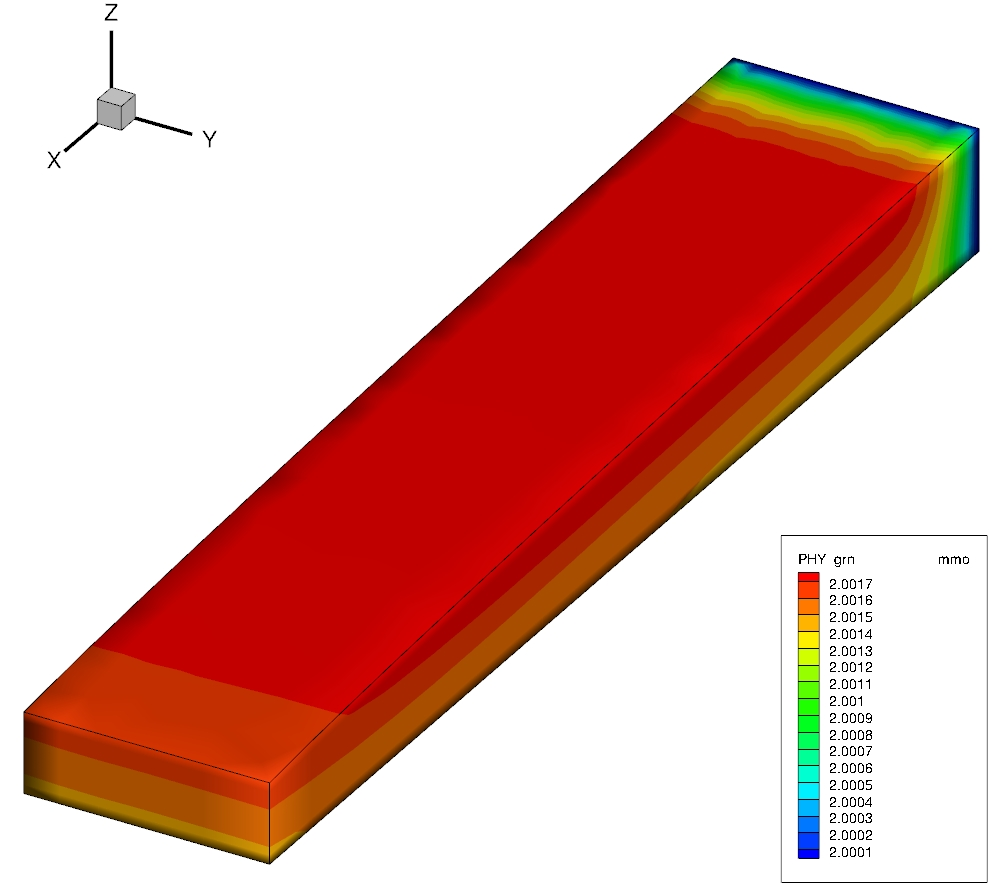
\includegraphics[scale=0.3]{flume_phyto.jpg}
\includegraphicsmaybe{[width=0.8\textwidth]}{../img/res_oxy.png}
\includegraphicsmaybe{[width=0.8\textwidth]}{../img/res_ammonium.png}
\includegraphicsmaybe{[width=0.8\textwidth]}{../img/res_nitrate.png}
\includegraphicsmaybe{[width=0.8\textwidth]}{../img/res_phosphate.png}
\includegraphicsmaybe{[width=0.8\textwidth]}{../img/res_dop.png}
\includegraphicsmaybe{[width=0.8\textwidth]}{../img/res_don.png}
 \caption{Vertical distribution of oxygen, ammonium, nitrate, phosphate, DOP, DON after 160~s}
 \label{fig:waq3d_aed2_flume:res}
\end{figure}
%
\section{Conclusion}
%
\telemac{3D} can be coupled with AED2 to model unsteady flows.
%
% Here is an example of how to include the graph generated by validate_telemac.py
% They should be in test_case/img
%\begin{figure} [!h]
%\centering
%\includegraphics[scale=0.3]{../img/mygraph.png}
% \caption{mycaption}\label{mylabel}
%\end{figure}
